\epigraph{``I've got a bad feeling about this"}{Hans Solo}

\section{Geostrophic Wind}\label{geostrophic_wind}
There are a number of forces that can either change the force or direction of wind. Two of the biggest forces of wind vectors are the pressure gradient force and the Coriolis force.

\subsection{Pressure-Gradient Force}
\begin{definition}
The pressure-gradient force is a force acting on air that is due to pressure differences.
\end{definition}

Horizontal variations in pressure create a tendency for movement from higher to lower pressure. The atmosphere, like all systems in nature, is trying to stay at the lowest energy level possible. Therefore, if there is an area of lower pressure nearby, air will freely move from the high pressure area to the low pressure area in order to equalise this energy gradient. To do this, it will attempt to take the shortest distance possible in order to maximise efficiency, which happens to be perpendicular to the isobars\cite{pressuregrad_def}. This phenomenon is described by equation \ref{pressure_grad}, where $P$ is the pressure-gradient force.

\begin{equation}
    \label{pressure_grad}
    P = - \Vec{\nabla} p
\end{equation}

The negative sign at the beginning of the equation designates that we move from high to low across the pressure gradient. The greater the difference in pressure between the two locations, the greater the pressure gradient. A stronger pressure-gradient force usually correlates to a stronger wind vector. It must be noted that the pressure-gradient force is only one component of the forces acting on the actual wind, though, so, air does not normally flow perpendicular to the isobars\cite{pressure_grad}.

\subsection{Coriolis Force}\label{f_section}
\begin{definition}
The Coriolis force is an inertial force that acts on objects that are in motion within a frame of reference that rotates with respect to an inertial frame.
\end{definition}

The Coriolis force ultimately results in the diversion of the wind's direction within the atmosphere due to the Earth's rotation. The Earth is spinning in a prograde direction. The Earth is a elongated spheroid, however, to a reasonable good approximation, it can be considered to be a sphere. Due to this fact, all points on the surface of the Earth are travelling at the same angular velocity. As a consequence, however, a point near the equator must have a higher linear velocity, as it must travel a larger distance than a point near the poles. When an object moves either closer or further from the equator its original momentum is preserved, giving the path a diversion off its original course\cite{corioliseffect_def}. If the wind is travelling in accordance with the pressure-gradient force, the wind will be deflected off its original course by the Coriolis force. It must be noted that there isn't a Coriolis force at the equator, however, it increases with intensity as one approaches the poles. The Coriolis force is described by equation \ref{coriolis_force}.

\begin{equation}
    \label{coriolis_force}
    F = \rho U f_0
\end{equation}

where $f_0$ is the Coriolis parameter, and is given by equation \ref{f}.

\begin{equation}
    \label{f}
    f_0 = 2 \Omega \sin{\phi}
\end{equation}

One can therefore deduce that the higher the latitude, the higher the Coriolis force. Also, the Coriolis force only acts on air that is already set into motion. The Coriolis force will not set wind into motion, but will only deflect the direction of wind that is already moving. Therefore, it follows that the faster that air is moving, the stronger it is affected by the Coriolis force\cite{coriolis_effect}. 

Equation \ref{f} is known as the f-plane approximation, which can be visualised as a tangent plane touching the surface of the sphere at this latitude. The beta plane approximation is, however, utilised in the quasi-geostrophic theory, which ignores the variation of $f$ with latitude. In this approximation, $f$ is set to vary linearly in space and a value of $f$ appropriate for a particular latitude is used throughout the domain. The equation describing the beta plane approximation is as follows:

\begin{equation}
    f = f_0 + \beta y
\end{equation}

The advantage of the beta plane approximation over more accurate formulations is that it does not contribute nonlinear terms to the dynamical equations\cite{beta_approx}. $\beta$ in the above equation is the Rossby number, which is discussed in the following section\cite{rossby_number}.

\subsection{Geostrophic Balance}\label{balance}
\begin{definition}
Geostrophic Balance is an exact balance between the Coriolis force and the pressure-gradient force.
\end{definition}

This balance seldom holds true in nature. This concept, however, will lead to the development of a theoretical wind, known as geostrophic wind. First and foremost, lets introduce the horizontal momentum equations.

\begin{equation}
    \frac{Du}{Dt} = -\frac{1}{\rho}\frac{\partial p}{\partial x} + f v
\end{equation}

\begin{equation}
    \frac{Dv}{Dt} = -\frac{1}{\rho}\frac{\partial p}{\partial y} - f  u
\end{equation}

Assuming geostrophic balance, the system is stationary and the first two equations become:  

\begin{equation}
    u = -\frac{1}{\rho f} \frac{\partial p}{\partial y}
\end{equation}

\begin{equation}
    v = \frac{1}{\rho f} \frac{\partial p}{\partial x}
\end{equation}

\begin{definition}
Geostrophic Wind is the wind that flows parallel to height contours or isobars resulting from an exact balance between the Coriolis force and the pressure-gradient force.
\end{definition}

The geostrophic wind vector can also be expressed in terms of the gradient of the geopotential on a surface of constant pressure. This is extremely useful as it also for the calculation of geostrophic wind through the utilisation of geopotential height. It also allows for the calculation of geostrophic wind in an isobaric co-ordinate system. Therefore, the above equations are rewritten as follows:

\begin{equation}
    u_g = -\frac{g}{f} \frac{\partial \Phi}{\partial y}
    \label{u_g}
\end{equation}

\begin{equation}
    v_g = \frac{g}{f} \frac{\partial \Phi}{\partial x}
    \label{v_g}
\end{equation}

Any spatial derivatives within this equation are replaced by a central difference approximation of the derivatives, which results in:

\begin{equation}
    u_g = -\frac{g}{f} \frac{\Delta \Phi}{2 \Delta y}
\end{equation}

\begin{equation}
    v_g = \frac{g}{f} \frac{\Delta \Phi}{2 \Delta x}
\end{equation}

For the geostrophic flow concept to work, the wind must not be changing speed (is unaccelerated or the acceleration is almost zero). The question remains whether geostrophic wind is a good approximation for the actual wind. The tendency for wind to be accelerated can be measured at various scales of circulation. Meanwhile, the Coriolis acceleration is only related to the speed of the object and its latitude. Thus, as the flow  approaches geostrophic the smaller the actual acceleration is relative to the Coriolis acceleration\cite{geo_wind}.

\begin{definition}
Rossby Number is the ratio of the total acceleration to the Coriolis acceleration.
\end{definition}

If the Rossby number is small (less than one), the geostrophic wind is a reasonably good approximation for geostrophic wind, neglecting the force of friction in this assumption. From table 3.1, generally the geostrophic wind is a good approximation if it is determined at a synoptic scale\cite{geo_wind}. 

\hfill

\begin{center}
\begin{tabular}{|c|c|c|} 
 \hline
 Scale of Circulation & Rossby Number & Yes / No \\
 \hline
 10,000 km & 0.01 & Yes \\
 \hline
 1,000 km & 0.1 & Yes \\
 \hline
 100 km & 1.0 & Not Really \\
 \hline
 10 km & 3.0 & No \\
 \hline
 1 km & 4.0 & No \\
 \hline
\end{tabular}\par
\bigskip
Table 3.1.: Is geostrophic wind a good approximation for the real wind?
\end{center}

\section{Pressure Thickness}\label{pressure_thickness}
\begin{definition}
Pressure Thickness is the measurement of the distance (in metres) between any two constant pressure surfaces.
\end{definition}

\begin{figure}[H]
    \centering
    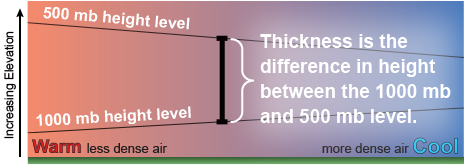
\includegraphics[width=.8\linewidth]{Images/thickness_def.png}
    \caption{Pressure Thickness Definition (provided by the NWS of the USA)}
    \label{thickness_def}
\end{figure}

One of the most common thickness charts used in meteorology is the 1000-500 hPa thickness, and for the purposes of this project, it will be the sole interest. This is the distance between the elevation of the 1,000 hPa and 500 hPa levels. Typically, the 1,000 hPa surface is used to represent sea level but this is just a generalisation. On pressure charts, the last digit (zero) of a thickness value is typically truncated. So, a 1000-500 thickness value of 570 means the distance between the two surfaces is 5,700 metres. The 1000-500 hPa thickness value of 540 is traditionally used to determine rain versus snow. If precipitation is predicted poleward of this 540-thickness line (if the thickness value is less than 540), it is expected that it will be snow. If precipitation is predicted on the equator side of this line (if the thickness value is greater than 540), then it is expected that the precipitation will be in a liquid form. The reason one is able to make such an expectation is due to the fact that the 540-thickness line closely follows the surface freezing temperature of 273 K\cite{thickness}.

\begin{figure}[H]
    \centering
    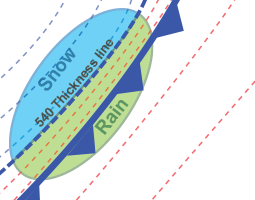
\includegraphics[width=.4\linewidth]{Images/rainsnow_line.png}
    \caption{Rain/Snow Line (provided by the NWS of the USA)}
    \label{rainsnow_line}
\end{figure}

To determine the pressure thickness between two constant pressure surfaces, the Hypsometric equation is utilised and as shown in equation \ref{hypsometric}. 

\begin{definition}
The hypsometric equation relates an atmospheric pressure ratio to the equivalent thickness of an atmospheric layer considering the layer mean of virtual temperature, gravity, and occasionally wind. It is derived from the hydrostatic equation and the ideal gas law.
\end{definition}

\begin{equation}
    \label{hypsometric}
    h = \Phi_2 - \Phi_1 = \frac{R \bar{T_v}}{g} \ln{\frac{p_1}{p_2}}
\end{equation}

\section{Precipitable Water}
\begin{definition}
Precipitable Water is the total atmospheric water vapour contained in a vertical column of unit cross-sectional area extending between any two specified pressure levels.
\end{definition}

Based on the definition, precipitable water can be described mathematically as being:

\begin{equation}
    \label{pwv_1}
    W = \int_{0}^{z} \rho_v dz
\end{equation}

where $\rho_v$ is the density of water vapour, and where $\rho_v$ is defined as:

\begin{equation}
    \rho_v = \frac{\texttt{mass of vapour}}{\texttt{unit volume}}
\end{equation}

Following which, the hydrostatic equation can be applied to equation \ref{pwv_1} in order to replace $dz$ with $dp$. The reason for doing this is that atmospheric pressure is extremely easier to measure, with devices such as weather balloons being readily available.

\begin{equation}
    \label{pwv_derive}
    W = -\int_{p_1}^{p_2} \frac{\rho_v}{\rho g} dp
\end{equation}

Where $p_1$ and $p_2$ are constant pressure surfaces, and where $p_1 > p_2$. Substituting in the definition of density, $\rho_v = \frac{m_v}{V}; \rho = \frac{m_{air}}{V}$, into equation \ref{pwv_derive} results in:

\begin{equation}
    W = -\int_{p_1}^{p_2} \frac{1}{g} \frac{m_v V}{m_{air} V} dp
\end{equation}

\begin{equation}
    \Rightarrow W = - \frac{1}{g} \int_{p_1}^{p_2} \frac{m_v}{m_{air}} dp
\end{equation}

The integration term in this particular equation is the definition for the specific humidity, with the units of measurement being $\frac{kg}{kg}$. The specific humidity can be approximated by the mixing ratio, with an error typically around 4 \%\cite{pwv_def}.

\begin{definition}
Mixing Ratio is the ratio of the mass of a variable atmospheric constituent to the mass of dry air.
\end{definition}

\begin{equation}
    \label{pwv_derive_fin}
    \therefore W = -\frac{1}{g} \int_{p_1}^{p_2} m dp
\end{equation}

The units as given by the equation are $\frac{kg}{m^2}$ (dimensionless), but, the preferred unit of measurement for rainfall is $mm$. The conversion between the two units of measurements is one to one ($1 \frac{kg}{m^2} = 1 mm$) In actual rainstorms, particularly thunderstorms, amounts of rain very often exceed the total precipitable water of the overlying atmosphere. This results from the action of convergence that brings into the rainstorm the water vapour from a surrounding area that is often quite large. Nevertheless, there is general correlation between precipitation amounts in given storms and the precipitable water of the air masses involved in those storms\cite{problems_with_pwv}.

For the purposes of numerically calculating the precipitable water for a given column of air, equation \ref{pwv_derive_fin} is commonly rewritten as the following:

\begin{equation}
    \label{pwv}
    W = -\frac{1}{\rho g} \int_{p_1}^{p_2} \frac{0.622 e}{p - e} dp
\end{equation}

\begin{definition}
Vapour Pressure is the pressure exerted by a vapour when the vapour is in equilibrium with the liquid or solid form, or both, of the same substance. In meteorology, vapour pressure is used almost exclusively to denote the partial pressure of water vapour in the atmosphere.
\end{definition}

Considering vapor pressure is not one of the three prognostic variables defined in section \ref{noaa_initial_conditions}, it is therefore necessary to express vapor pressure in terms of the already defined variables. This can be done through the utilisation of temperature and relative humidity. First, one must determine the saturated vapour pressure. This can be done using the following equation\cite{balton}:

\begin{equation}
    e_s = 6.112 \exp(\frac{17.67 T}{T + 243.5})
\end{equation}

After which, the vapor pressure can be calculated as follows:

\begin{equation}
    e = \frac{e_{s} r}{100}
    \label{vapor_pressure_eq}
\end{equation}

In wet periods, the precipitable water is particularly close to the saturated precipitable water. In situations when the precipitable water is close to the saturated precipitable water, the precipitable water changes very little over the day. Saturated precipitable water also makes calculations a whole lot simpler, as specific humidity data is rather difficult to come by.

In regards to the numerical calculation of the precipitable water, the SciPy method, scipy.integrate.quad, is utilised in order to determine the definite integral in equation \ref{pwv}. This method integrates the function using a technique from the Fortran library, QUADPACK\cite{scipy_integrate}. 

\section{Virtual Temperature}\label{virtual_section}
The virtual temperature is the temperature at which dry air would have the same density as the moist air, at a given pressure. In other words, two air samples with the same virtual temperature have the same density, regardless of their actual temperature or relative humidity. Because water vapor is less dense than dry air and warm air is less dense than cool air, the virtual temperature is always greater than or equal to the actual temperature. 

In relation to this project, the virtual temperature will be extremely useful as it will allow for the calculation of the evolution of relative humidity through the utilisation of the thermodynamic advection equation (which is discussed in section \ref{advection_equation}). This is due to the fact that virtual temperature can be expressed in terms of vapor pressure, which can be converted into relative humidity.  This can be seen as follows:

\begin{equation}
    T_v = \frac{T}{1 - \frac{0.378 e}{p}}
\end{equation}

The equation becomes the following, by substituting equation \ref{vapor_pressure_eq} in and rearranging for relative humidity:

\begin{equation}
    r = \frac{100 (p T_v - p T)}{0.378 e_s T_v}
\end{equation}

\section{Quasi-Geostrophic Theory}
\subsection{Introduction}
From numerical weather prediction, the public desires information pertaining to the temperature, wind speed, wind direction and humidity in their area up to 7 days in advance. This information is largely a function of evolving synoptic weather patterns (for example, fronts and jet streams). The basic idea of quasi-geostrophic theory is that it reveals how hydrostatic balance and geostrophic balance constrain and simply atmospheric dynamics, but, in a realistic manner. It provides a framework by which an understanding of, and an ability to diagnose, the evolution of a three dimensional synoptic-scale weather system. It achieves this by providing insights into how mass fields and momentum fields interact to create vertical circulations that result in realistic synoptic-scale weather patterns.

\subsection{Thermodynamic Equation}\label{advection_equation}
To begin with, the thermodynamic equation will be the primary focus. The first thing to examine in the thermodynamic equation is advection. As mentioned previously, advection is a horizontal transfer of mass, heat, or other property. Accordingly, winds that blow across Earth's surface represent advectional movements of air. 

Differential temperatures drive the mass movement of air seeking equilibrium. Advective winds move from areas of higher temperature toward areas of lower temperature. In contrast, convection, the vertical movement of mass or transfer of heat, manifests itself as air currents. Accordingly, winds are a result of advection, while air currents are a result of convection. In the atmosphere, advection is the sole process of horizontal transfer of mass. In contrast, vertical transfer occurs via conduction, convection, and radiation.

The magnitude of heat transference depends on the rate of heat transport, and flux in turn relates the transfer of heat energy in terms of area and time\cite{advection}. Advection can be represented in vector notation by:

\begin{equation}
    \frac{\partial T}{\partial t} + \Vec{v} \cdot \nabla_p T = 0
\end{equation}

The del operator ($\nabla_p$) will be expanded into its components as shown in equation \ref{del_operator}. The reason for doing so is that it makes the equation easier to work with down the line.

\begin{equation}
    \Rightarrow \frac{\partial T}{\partial t} + \begin{bmatrix} \Vec{v}_x \\ \Vec{v}_y \\ \Vec{v}_p \end{bmatrix} \cdot \begin{bmatrix} \frac{\partial}{\partial x} \hat{i} \\ \frac{\partial}{\partial y} \hat{j} \\ \frac{\partial}{\partial p} \hat{k} \end{bmatrix} T
    \label{del_operator} = 0
\end{equation}

Taking the dot product results in the following:

\begin{equation}
     \frac{\partial T}{\partial t} = - (\Vec{v_{x}} \frac{\partial}{\partial x} \hat{i} + \Vec{v_{y}} \frac{\partial}{\partial y} \hat{j} + \Vec{v_{p}} \frac{\partial}{\partial p} \hat{k}) T
\end{equation}

Expanding the brackets results in:

\begin{equation}
     \frac{\partial T}{\partial t} = -\Vec{v_{x}} \frac{\partial T_{x}}{\partial x} - \Vec{v_{y}} \frac{\partial T_{y}}{\partial y} - \Vec{v_{p}} \frac{\partial T_{p}}{\partial p} 
\end{equation}

\begin{equation}
    \Rightarrow \frac{\partial T}{\partial t} = -u \frac{\partial T}{\partial x} - v \frac{\partial T}{\partial y} - \omega \frac{\partial T}{\partial p}
\end{equation}

The terms on the RHS are due to advection within the atmosphere. Each $T$ is actually different and related to its respective plane. This is divided by the distance between grid points to get the change in temperature with the change in distance. When multiplied by the wind velocity on that plane, the units $K m^{-1}$ and $m s^{-1}$ give $K s^{-1}$. The sum of all the changes in temperature due to motions in the $x$, $y$, and $p$ directions give the total change in temperature with time\cite{primitive_equations}.

This is the almost complete version of the thermodynamic equation, however, it is also necessary to add an additional term for vertical transfer, hence, the above equation becomes the following:

\begin{equation}
    \Rightarrow \frac{\partial T}{\partial t} = -u \frac{\partial T}{\partial x} - v \frac{\partial T}{\partial y} - \omega \frac{\partial T}{\partial p} + \omega \frac{R T}{p c_p}
\end{equation}

It is then possible to combine the two terms containing vertical motion resulting in:

\begin{equation}
    \Rightarrow \frac{\partial T}{\partial t} = -u \frac{\partial T}{\partial x} - v \frac{\partial T}{\partial y} + \omega \sigma \frac{p}{R}
    \label{analytic_temp_final}
\end{equation}

This equation describes temperature changing at a particular location and height is a function of temperature advection and vertical motion. Warm advection causes a temperature increase. Ascent causes adiabatic cooling and a temperature decrease, while descent produces adiabatic heating. These two terms often oppose each other. 

\begin{definition}
Adiabatic cooling is the process of reducing heat through a change in air pressure caused by volume expansion.
\end{definition}

For example, strong warm advection at a level causes local warming, but often ascent as well. The ascent leads to adiabatic cooling opposing the warming due to warm advection. Given strong ascent, this can contribute to isotherms (lines on a weather showing areas of equal temperature) remaining steady or even sinking southward in the face of warm advection, which may be very important for heavy precipitation production. Models can show this process, which likely will be accompanied by areas of strong model upward motion. In borderline precipitation phase change situations, the absence of strong ascent can result in, for example, drizzle. However, if a burst of vertical motion develops in this area, strong adiabatic cooling can temporary cause a phase change to snow, with precipitation diminishing and changing back to liquid once the enhanced ascent zone moves away\cite{describe_quasi}.

Discretizing equation \ref{analytic_temp_final}, by the method described in section \ref{fdm_section} results in:

\begin{equation}
    \frac{T^{n + 1}_{x, y, z} - T^{n - 1}_{x, y, z}}{2 \Delta t} = -u \frac{T^{n}_{x+1, y, z} - T^{n}_{x-1, y, z}}{2 \Delta x} - v \frac{T^{n}_{x, y+1, z} - T^{n}_{x, y-1, z}}{2 \Delta y} + \omega \sigma \frac{p}{R}
\end{equation}

Multiplying both the LHS and the RHS by $2 \Delta t$ in order to isolate the change in temperature with respect to time term results in the following:

\begin{equation}
     T^{n + 1}_{x, y, z} - T^{n - 1}_{x, y, z} = - u \frac{2 \Delta t}{2 \Delta x} (T^{n}_{x+1, y, z} - T^{n}_{x-1, y, z}) - v \frac{2 \Delta t}{2 \Delta y} (T^{n}_{x, y+1, z} - T^{n}_{x, y-1, z}) + \omega \sigma \frac{p}{R}
\end{equation}

Rearranging the equation in order to isolate the $T^{n + 1}_{x, y, z}$ term: 

\begin{equation}
     T^{n + 1}_{x, y, z} = T^{n - 1}_{x, y, z} - u \frac{2 \Delta t}{2 \Delta x} (T^{n}_{x+1, y, z} - T^{n}_{x-1, y, z}) - v \frac{2 \Delta t}{2 \Delta y} (T^{n}_{x, y+1, z} - T^{n}_{x, y-1, z}) + \omega \sigma \frac{p}{R}
\end{equation}

This discretized equation will allow for the calculation of the evolution of temperature and virtual temperature. Hence, this will also allow for the calculation of the evolution of relative humidity as described in section \ref{virtual_section}.

\subsection{Height Tendency Equation}
In order to predict system evolution, it is necessary to examine changes in the local height field. Therefore, the goal is to develop a single prognostic equation for geopotential height. Although the vertical velocity plays an essential role in the dynamics, the evolution of the geostrophic circulation can be determined without explicitly determining the distribution of the vertical velocity\cite{eq_describe}. To do this, it is necessary to begin with the definition of geostrophic relative vorticity:

\begin{equation}
    \zeta_g = \frac{\partial v_g}{\partial y} - \frac{\partial u_g}{\partial x}
    \label{zeta}
\end{equation}

The relative vorticity is the vorticity (a measure of the local rotation of a fluid) relative to the Earth induced by the air velocity field. In the case of geostrophic relative vorticity, the air velocity field would be the geostrophic wind. This air velocity field is modelled as a two-dimensional flow parallel to the ground, so that the relative vorticity vector is generally a scalar rotation quantity perpendicular to the ground. Vorticity is positive, when looking down on the Earth and when the wind is turning counterclockwise\cite{vorticity}. The following can be shown, by, substituting equations \ref{u_g} and \ref{v_g} into equation \ref{zeta}:

\begin{equation}
    \zeta_g = \frac{1}{f_0} \nabla^{2}_p \varphi      
\end{equation}

\begin{definition}
Geopotential is the potential of the Earth's gravity field. For convenience it is often defined as the negative of the potential energy per unit mass, so that the gravity vector is obtained as the gradient of this potential, without the negation.
\end{definition}

Redefining the hydrostatic equation in section \ref{hydro_balance} in isobaric coordinates results in the following:

\begin{equation}
    g \frac{\partial \Phi}{\partial p} = - \frac{R T}{p}
\end{equation}

Using the definition of geopotential $\varphi = g \Phi$, it is possible to rearrange the above equation in terms of temperature:

\begin{equation}
    T = - \frac{p}{R} \frac{\partial \varphi}{\partial p}    
\end{equation}

It is now possible to define local changes in vorticity and temperature in terms of the local height tendency on constant pressure surfaces:

\begin{equation}
    \frac{\partial \zeta_g}{\partial t} = \frac{\partial}{\partial t} (\frac{1}{f_0} \nabla^{2}_p \varphi) = \frac{1}{f_0} \nabla^{2}_p \frac{\partial \varphi}{\partial t}
\end{equation}

\begin{equation}
    \frac{\partial T}{\partial t} = \frac{\partial}{\partial t} (- \frac{p}{R} \frac{\partial \varphi}{\partial p}) = - \frac{p}{R} \frac{\partial (\frac{\partial \varphi)}{\partial t}}{\partial p} 
\end{equation}

For compactness, $\frac{\partial \varphi}{\partial t}$ will be defined as $\varphi_t$, therefore, the above equations become:

\begin{equation}
    \frac{\partial \zeta_g}{\partial t} = \frac{1}{f_0} \nabla^{2}_p \varphi_t
    \label{zeta_relationship}
\end{equation}

\begin{equation}
    \frac{\partial T}{\partial t} = - \frac{p}{R} \frac{\partial \varphi_t}{\partial p} 
\end{equation}

These two relationships are very powerful and will be used to physically interpret the terms in the height tendency. It is now possible to substitute the new relationship for temperature into the thermodynamic equation, which results in:

\begin{equation}
    - \frac{p}{R} \frac{\partial \varphi_t}{\partial p} = -u \frac{\partial T}{\partial x} - v \frac{\partial T}{\partial y} + \omega \sigma \frac{p}{R}
\end{equation}

It is also possible to substitute the vorticity relationship into something known as the quasi-geostrophic vorticity equation. This equation is mathematically defined as the following:

\begin{equation}
    \frac{\partial \zeta_g}{\partial t} = -u \frac{\partial \zeta_g}{\partial x} - v \frac{\partial \zeta_g}{\partial y} + f_0 \frac{\partial \omega}{\partial p} - \beta v_g
\end{equation}

This equation states that vorticity changes at a location are due to vorticity advection and vertical divergence. Positive vorticity advection causes geostrophic relative vorticity to increase with time. A vertical divergence results in a vorticity increase. It is, therefore, possible to see how positive vorticity advection and negative vorticity advection affect vorticity at a point\cite{describe_quasi}. Therefore, substituting the relationship established in equation \ref{zeta_relationship} into the quasi-geostrophic vorticity equation results in:

\begin{equation}
    \frac{1}{f_0} \nabla^{2}_p \varphi_t = -u \frac{\partial \zeta_g}{\partial x} - v \frac{\partial \zeta_g}{\partial y} + f_0 \frac{\partial \omega}{\partial p} - \beta v_g
\end{equation}

It is now possible to derive a single prognostic equation for geopotential (diagnostic equation for $\varphi_t$)\cite{quasi_geo}. To do this, it is necessary to eliminate the vertical motion from both equations by:

\begin{enumerate}
    \item Apply the operator $-\frac{f^{2}_0}{\sigma} \frac{\partial}{\partial p} (\frac{R}{p})$ to the thermodynamic equation.
    \item Multiply the quasi-geostrophic vorticity equation by $f_0$.
    \item Add the results of the two proceeding steps.
\end{enumerate}

After a lot of tedious mathematics, the following diagnostic equation is obtained:

\begin{equation}
    (\nabla^2_p + \frac{f^2_0}{\sigma} \frac{\partial^2}{\partial p^2}) \varphi_t = - f_0 \Vec{v_g} \cdot \nabla_p (\zeta_g + f) - \frac{f^2_0}{\sigma} \frac{\partial}{\partial p} (\frac{R}{p} (-\Vec{v_g} \cdot \nabla_p T))
    \label{complex_qg}
\end{equation}

To obtain an actual value for $\varphi_t$, it would be necessary to compute the forcing terms from the three-dimensional wind and temperature fields, and then invert the operator on the LHS using appropriate boundary conditions. This is not a simple task, and forecasters never do this. Rather, for synoptic-scale atmospheric waves, this term is proportional to $-\varphi_t$. This term can be as the local geopotential tendency\cite{quasi_geo}. Therefore, equation \ref{complex_qg} becomes the following:

\begin{equation}
    - \varphi_t = - f_0 \Vec{v_g} \cdot \nabla_p (\zeta_g + f) - \frac{f^2_0}{\sigma} \frac{\partial}{\partial p} (\frac{R}{p} (-\Vec{v_g} \cdot \nabla_p T))
\end{equation}

\begin{equation}
    \Rightarrow \varphi_t = f_0 \Vec{v_g} \cdot \nabla_p (\zeta_g + f) + \frac{f^2_0}{\sigma} \frac{\partial}{\partial p} (\frac{R}{p} (-\Vec{v_g} \cdot \nabla_p T))
\end{equation}

\begin{equation}
    \Rightarrow \frac{\partial \varphi}{\partial t} = \underbrace{f_0 \Vec{v_g} \cdot \nabla_p (\zeta_g + f)}_{\texttt{Term A}} + \underbrace{\frac{f^2_0}{\sigma} \frac{\partial}{\partial p} (\frac{R}{p} (-\Vec{v_g} \cdot \nabla_p T))}_{\texttt{Term B}}
    \label{complex_qg_proportional}
\end{equation}

Term A is proportional to the advection of absolute vorticity. For the upper troposphere it is usually the dominant term.
For short waves we have seen that the relative vorticity advection dominates the planetary vorticity advection. Term B is proportional to minus
the rate of change of temperature advection with respect to pressure. It is therefore related to plus the rate of change of temperature advection with respect to height. This is called the differential temperature advection. The magnitude of the temperature advection tends to be largest in the lower troposphere\cite{describe_quasi}.

In order to allow for numerical computation, it is necessary to discretize (the discretization process is described in great depth in section \ref{fdm_section}). Based on this, term A becomes the following:

\begin{equation}
    A = f_0 \Vec{v_g} \cdot \nabla_p (\zeta_g + f)
\end{equation}

\begin{equation}
    \Rightarrow A = f_0 (u_g \frac{\partial (\zeta_g + f)}{\partial x} + v_g \frac{\partial (\zeta_g + f)}{\partial y})
\end{equation}

\begin{equation}
    \Rightarrow A = f_0 u_g \frac{\partial (\zeta_g + f)}{\partial x} + f_0 v_g \frac{\partial (\zeta_g + f)}{\partial y}
\end{equation}

\begin{equation}
    \Rightarrow A = f_0 u_g \frac{(\zeta_g + f)^{n}_{x+1, y, z} - (\zeta_g + f)^{n}_{x-1, y, z}}{2 \Delta x} + f_0 v_g \frac{(\zeta_g + f)^{n}_{x, y+1, z} - (\zeta_g + f)^{n}_{x, y-1, z}}{2 \Delta y}
\end{equation}

By a similar process, term B becomes the following:

\begin{equation}
    B = \frac{f^2_0}{\sigma} \frac{\partial}{\partial p} (\frac{R}{p} (-u_g \frac{\partial T}{\partial x} - v_g \frac{\partial T}{\partial y}))
\end{equation}

\begin{equation}
    \Rightarrow B = \frac{f^2_0}{\sigma} \frac{1}{ 2 \Delta p} (\frac{R}{p} (-u_g \frac{T^{n}_{x+1, y, z} - T^{n}_{x-1, y, z}}{2 \Delta x} - v_g \frac{T^{n}_{x, y+1, z} - T^{n}_{x, y-1, z}}{2 \Delta y})
\end{equation}

Substituting these discretized terms into equation \ref{complex_qg_proportional}, it becomes the following after following a similar discretization process:

\begin{equation}
    \frac{\partial \varphi}{\partial t} = A + B
\end{equation}

\begin{equation}
    \Rightarrow \frac{\varphi^{n+1}_{x, y, z} - \varphi^{n-1}_{x, y, z}}{2 \Delta t} = A + B
\end{equation}

\begin{equation}
    \Rightarrow \varphi^{n+1}_{x, y, z} - \varphi^{n-1}_{x, y, z} = 2 \Delta t(A + B)
\end{equation}

\begin{equation}
    \Rightarrow \varphi^{n+1}_{x, y, z} = \varphi^{n-1}_{x, y, z} + 2 \Delta t(A + B)
\end{equation}

This discretized equation now allows for the computation of the evolution of geopotential. By using the definition of geopotential $\varphi = g \Phi$, it is possible to determine the geopotential height by rearranging the equation to $\Phi = \frac{\varphi}{g}$, which in turns allows for the computation of the geostrophic wind as described in section \ref{geostrophic_wind}\cite{quasi_geo}.
